\documentclass{article}
\usepackage{hyperref}
\usepackage[utf8]{inputenc}
\usepackage[english,polish]{babel}
\usepackage{polski}
\usepackage{graphicx}
\graphicspath{ {./} }

\title{Office Space Manager}
\author{Dokumentacja}
\date{22 Listopad 2021}

\begin{document}

\maketitle

\section{Lista członków projektu}
\begin{enumerate}
  \item Grzegorz Nieużyła
  \item Dawid Karolewski
\end{enumerate}


\section{Wprowadzenie}
Ciągle rosnąca liczba nowo zakładanych firm oraz rozwój obecnych stwarzają potrzebę sprawnego zarządzania powierzchnią biurową firm. W dobie automatyzacji wielu dziedzin i procesów, zarządzanie biurem nie jest tu wyjątkiem. Systemy te potrafią sprawnie zarządzać powierzchnią biurową bez zbytniej ingerencji człowieka i redukując wiele istotnych problemów, które wiążą się z procesem rezerwacji np. kolizje. Odpowiedzią na tego typu problemy i automatyzacja jest nasz system.
Dokumentacja obejmuje zakres: najważniejszych funkcjonalności, które system będzie posiadał, problemów, które trzeba będzie rozwiązać, ograniczeń różnego rodzaju (sprzętowe, budżetowe, czasowe i softwarowe). Omówiona zostanie przyjęta metodologia działania oraz założenia architektoniczne jakie przyjęto. Kolejne dwa rozdziały są kluczowe, ponieważ dokładnie omawiają architekturę, przepływ danych, strukturę bazy danych oraz wszelkiego rodzaju diagramy UML klas oraz aktywności, a także komponentów UI. Ostatni rozdział poświęcony jest słownikowi kluczowych pojęć biznesowych, które są konieczne do właściwego zrozumienia funkcjonowania systemu.


\section{Funkcjonalność systemu}
\begin{itemize}
  \item Możliwość rezerwacji, modyfikacji oraz usunięcia rezerwacji miejsca do pracy w wybranym slocie czasowym
  \item Inteligenty wybór bliskiego pomieszczenia w zależności od dokonanych rezerwacji przez ludzi w danym zespole
  \item Powiadomienia mailowe o stanie rezerwacji
  \item Zapis do pliku istotnych informacji o rezerwacji, bądź raportu z nich danego dnia
  \item Gromadzenie statystyk z zarządzania powierzchnia biurową
  \item Dodawanie komentarzy do danej rezerwacji w celu dyskusji pewnych szczegółów związanych z miejscem
  \item Możliwość deklaracji dodatkowego wyposażenia na rezerwowanym stanowisku/pomieszczeniu
\end{itemize}


\section{Problemy do rozwiązania}
\begin{itemize}
  \item Zarządzanie wyświetlanym kontentem dla różnego rodzaju użytkowników (role) 
  \item Nieprzerwana responsywność interfejsu użytkownika oraz dynamiczna aktualizacja danych w komunikacji z API na stronie
  \item Stworzenie optymalnego algorytmu do znajdowania miejsc na podstawie kodu zespołu
  \item Bezpieczeństwo aplikacji oraz zarządzanie dostępnością do systemu
  \item Zaprojektowanie sensownej struktury bazy danych
\end{itemize}


\section{Ograniczenia}

\subsection{Sprzętowe}
Brak ograniczeń. Projekt systemu nie wymaga specjalistycznego sprzętu lub niestandardowych zasobów do obliczeń oraz pamięci do gromadzenia danych. Być może w przyszłości konieczna będzie migracja, gdy aplikacja się rozwinie i będzie musiała gromadzić znacznie większe pokłady danych.

\subsection{Softwarowe}
Brak ograniczeń. Plan realizacji zakłada pozyskanie licencji do oprogramowanie IDE, a wszystkie inne biblioteki wykorzystane do konstrukcji systemu są darmowe.

\subsection{Budżetowe}
\begin{itemize}
  \item Możliwe zatrudnienie tylko dwóch programistów w obecnym budżecie
  \item Wykonanie podstawowej wersji systemu, bez bardzo zaawansowanych i wymyślnych funkcjonalności
\end{itemize}

\subsection{Czasowe}
\begin{itemize}
  \item Angaż programistów w innych projektach, co prowadzi do ciągłej zmiany kontekstu oraz zmniejszeniu czasu w tym projekcie
  \item Ukończenie podstawowego scope'u projektu w czasie 2 mieniący
\end{itemize}


\section{Przyjęta metodologia}
W projektowaniu i implementacji systemu wykorzystaliśmy metodykę kaskadową, ze względu na z góry zdefiniowany i narzucony rytm i charakter pracy. Metodologia ta zakłada, że następujące po sobie fazy:
\begin{itemize}
  \item Planowanie i specyfikacja wymagań
  \item Analiza systemu
  \item Projektowanie systemu
  \item Implementacja
  \item Testowanie
  \item Wdrożenie
\end{itemize}
występują po sobie bezpośrednio, ale dopiero wtedy kiedy zakończy się poprzednia. Sposób ten nie przewiduje również powrotu lub powtarzania w/w faz.


\section{Założenia architektoniczne}
\begin{itemize}
  \item Niezależność od systemu operacyjnego
  \item Brak konieczność instalowania dodatkowego oprogramowania poza przeglądarką internetową
  \item Administrator tworzy konto użytkownikowi - brak konieczności rejestracji, tylko logowanie do systemu
\end{itemize}


\section{Rys architektoniczny systemu}
Przedstawione zostaną trzy podstawowe diagramy nakreślające ogólny zarys sytemu, począwszy od ogólnej architektury systemu, poprzez diagram aktywności, kończąc na diagramie przepływu danych.

\subsection{Ogólna architektura systemu}
\hspace*{-3cm}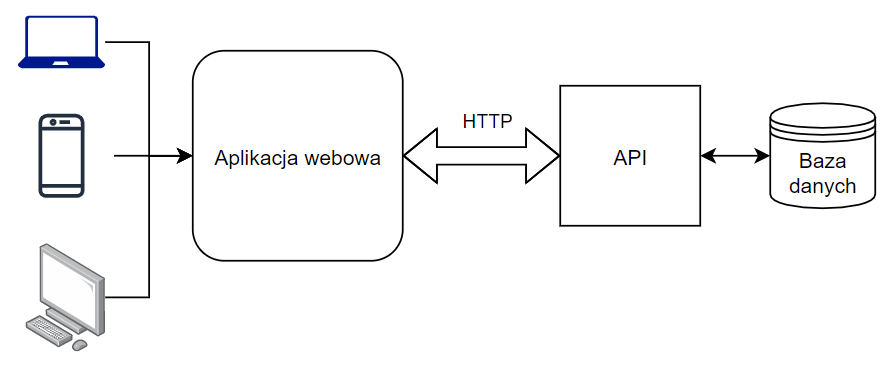
\includegraphics[scale=0.8]{architecture}
\begin{center}\textbf{Rys.1} Ogólna architektura systemu \end{center}
Użytkownik poprzez frontend (przyciski, formularze itp.) aplikacji w przeglądarce wyzwala akcje, które poprzez ruch HTTP powodują wysłanie żądań do backendu aplikacji (API). Następnie API przetwarza żądanie często manipulując przy tym bazą danych i po przygotowaniu odpowiedzi wysyła ją z powrotem, która jest wyświetlana użytkownikowi w odpowiedni sposób przez UI aplikacji webowej.

\subsection{Diagram aktywności}
\hspace*{-3cm}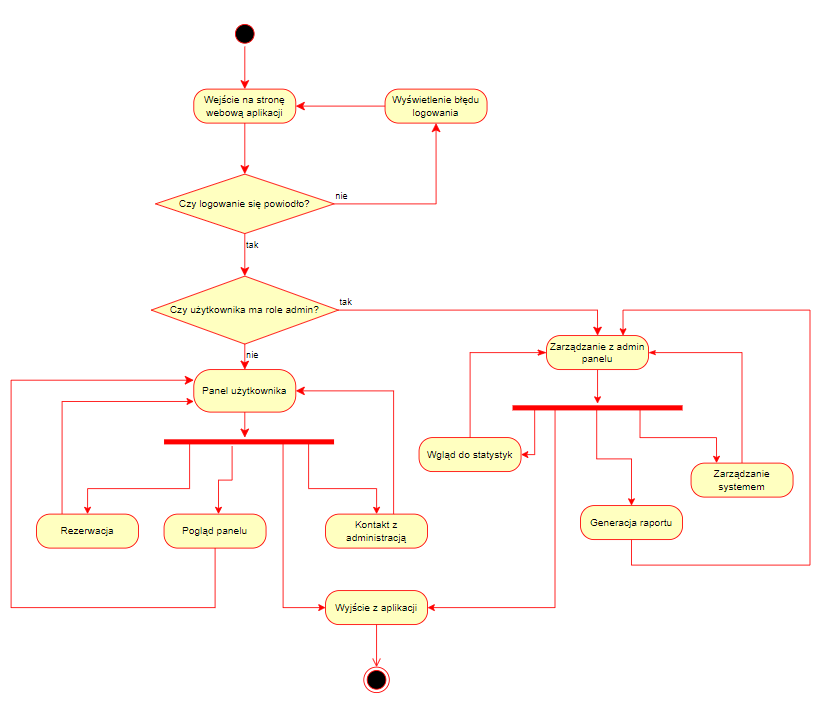
\includegraphics[scale=0.8]{activity_diagram}
\begin{center}\textbf{Rys.2} Diagram aktywności \end{center}
Po wejściu na stronę webową aplikacji użytkownik widzi ekran logowania. Po podaniu prawidłowego loginu i hasła przechodzi do strony głównej systemu. Jeśli weryfikacja poprawności loginu lub hasła się nie powiedzie wyświetlana jest komunikat o błędzie. Następnie system sprawdza wewnętrznie jaką rolę ma logujący się użytkownik i serwuje mu na tej podstawie odpowiedni dla admina - admin panel, a dla użytkownika - panel użytkownika. Użytkownik ma w tym momencie do wyboru rezerwację miejsca, podgląd obecnej rezerwacji wraz z sekcją komentarzy, a także może wysłać mail do administracji w razie problemów. Natomiast admin ma do wglądu statystyki funkcjonowania systemu, generacje tygodniowego raportu z rezerwacji oraz ogólne zarządzanie systemem (np. dodawanie użytkowników).

\subsection{Diagram przepływu danych}
\hspace*{-3.5cm}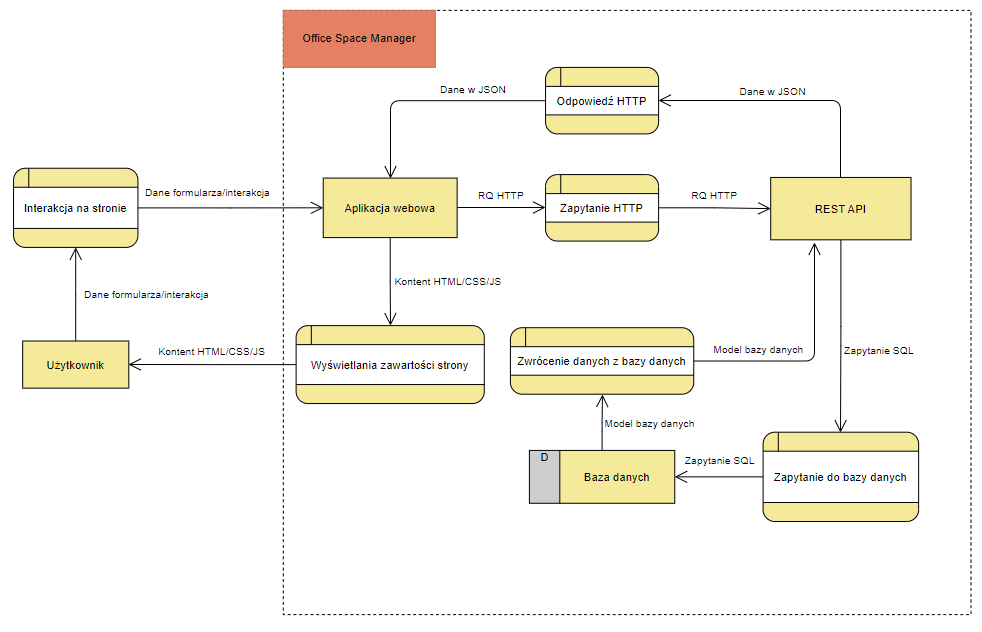
\includegraphics[scale=0.7]{dfd_diagram}
\begin{center}\textbf{Rys.3} Diagram przepływu danych \end{center}
Użytkownik jest głównym inicjatorem w systemie. Poprzez kliknięcie przycisków, wypełnienia formularzy, wysyłanie maili, pisania komentarzy wyzwala czynności w aplikacji webowej. Aplikacja na podstawie interakcji użytkownika wystosowuje zadanie HTTP do REST API, które zgodnie z logiką biznesową przetwarza dane i w razie potrzeby wysyła zapytanie SQL do bazy danych, która zwraca model bazy danych. Następnie REST API przetwarza dane i wykonuje zdefiniowane akcje. REST API wysyła jeśli żądanie tego wymagało odpowiedź w formacie JSON do aplikacji webowej, które formatuje dane i wyświetla użytkownikowi poprzez kontent HTML/CSS/JS za pomocą komponentów Reactowych.

\subsection{Diagram stanów rezerwacji}
\hspace*{-4cm}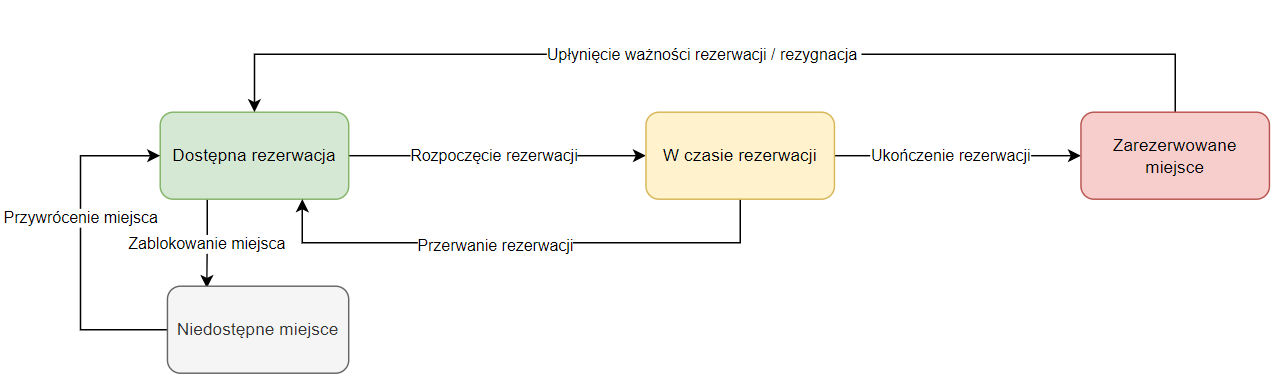
\includegraphics[scale=0.55]{state_diagram}
\begin{center}\textbf{Rys.4} Diagram stanów rezerwacji \end{center}
Jedynym diagramem stanów jest diagram stanów rezerwacji. Użytkownik jeśli dane miejsce jest wolne może dokonać rezerwacji i zrezygnować w niej w trakcie. Po dokonaniu rezerwacji, staje się ona niedostępna dla innych użytkowników, aż do momentu upłynięcia ważności rezerwacji lub rezygnacji. Administrator może też wyłączyć z użycia dane miejsce do rezerwacji oraz przywrócić jeśli znowu będzie dostępne.

\section{Szczegółowa architektura}

\subsection{Diagram UML klas}
\hspace*{-3cm}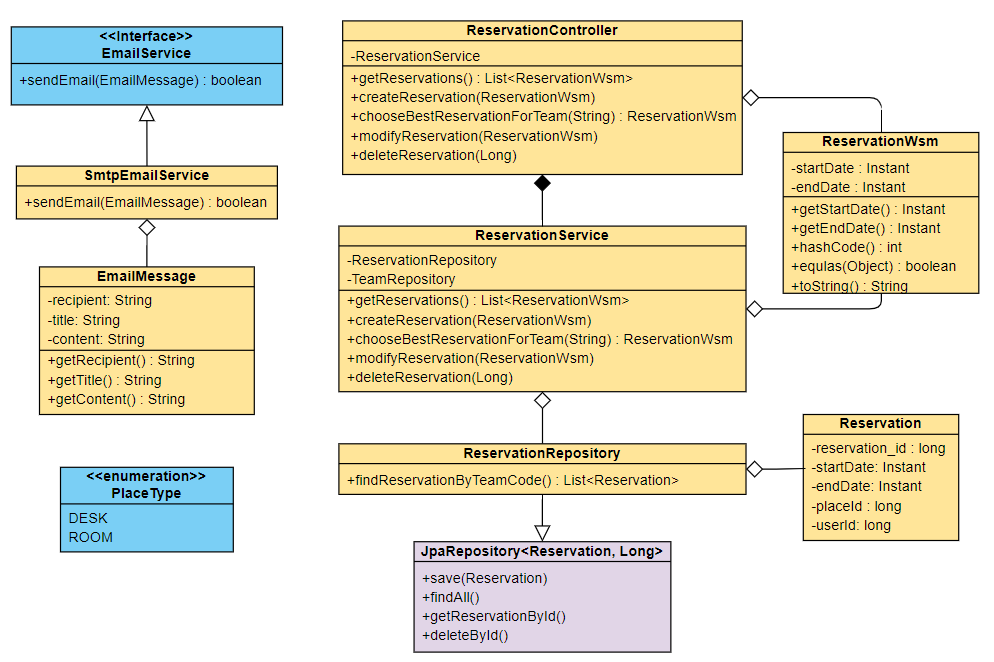
\includegraphics[scale=0.7]{uml_diagram}
\begin{center}\textbf{Rys.5} Diagram UML klas \end{center}
Przedstawiono wybrany model MVC na przykładzie modułu rezerwacji, ponieważ każdy inny moduł ma taką samą strukturę. Różni się tylko metodami, które są w znacznej większości analogiczne. Kontroler obsługuje żądania, które wystosowuję aplikacja webowa, a następnie wywołuję logikę biznesową zawartą w serwisie. Serwis korzysta w jednego lub wielu repozytoriów, które dostarczają bezpośrednio danych modelowych (Reservation) zwracanych z bazy danych. Repozytoria rozszerzają funkcjonalności JpaRepository. Klasy ReservationWsm to modele, które są spreparowane w formacie JSON i są używane w interakcji między kontrolerem, a aplikacją webową. Jedynym osobnym modułem, które nie implementuje wzorca projektowego MVC jest funkcjonalności wysyłania maili. Składa się ona z interfejsu, który został dodany, żeby pozostawić możliwość rozwoju aplikacji o inne serwisy mailowe. W pierwszej wersji systemu jedyną implementacją jest serwis mailowy SMTP, który korzysta z klasy EmailMessage, która definiuje strukturę wysyłanej wiadomości.System zawiera także enumy, do których najważniejszych należy rodzaj roli (admin, użytkownik), oraz rodzaj miejsca (pokój, biurko).

\subsection{Diagram komponentów UI}
\hspace*{-0.5cm}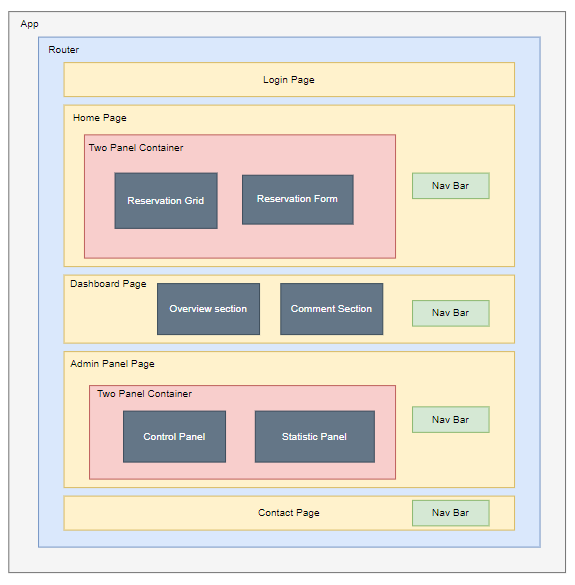
\includegraphics[scale=0.8]{components_diagram}
\begin{center}\textbf{Rys.6} Diagram komponentów UI \end{center}
Główny komponent aplikacji zamieszczony w DOM składa się klasycznie z Routera, który odpowiednio kieruje ruch na odpowiednią stronę. Początkowo do ekranu logowania, a następnie możemy nawigować się po aplikacji za pomocą komponentu Nav Bar. Admin Panel Page jest wyświetlana tylko dla użytkownika z rolą admina, a reszta stron jest przeznaczona do użytku przez normalnego użytkownika. Admin Panel Page oraz Home Page zawiera w sobie Two Panel Container, które dzieli stronę na prawą i lewą stronę. w Home Page mamy do dyspozycji dwa główne komponenty Reservation Grid, który jest siatką miejsc dla danego piętra oraz Reservation Form, który jest formularzem rezerwacji, w którym wybieramy datę rezerwacji, dodatkowe wyposażenie i specyfikujemy czy chcemy otrzymywać maila przypominającego o rezerwacji. Dashboard Page zawiera sekcję komentarzy - Comment Section do danej rezerwacji oraz Overview Section, które prezentuje obecny stan rezerwacji naszej. W Admin Panel Page administrator ma do dyspozycji panel ze statystykami - Statistic Panel oraz Control Panel, który zawiera możliwość generacji raportu oraz udostępnia np. dodawanie użytkowników. Contact Page, zawiera podstawowe informacje kontaktowe w razie problemów z system, które miałby użytkownik oraz udostępnia link, który przekierowuję automatycznie do wysyłania maila na supportowy mail.

\subsection{Diagram struktury bazy danych}
\hspace*{-1.5cm}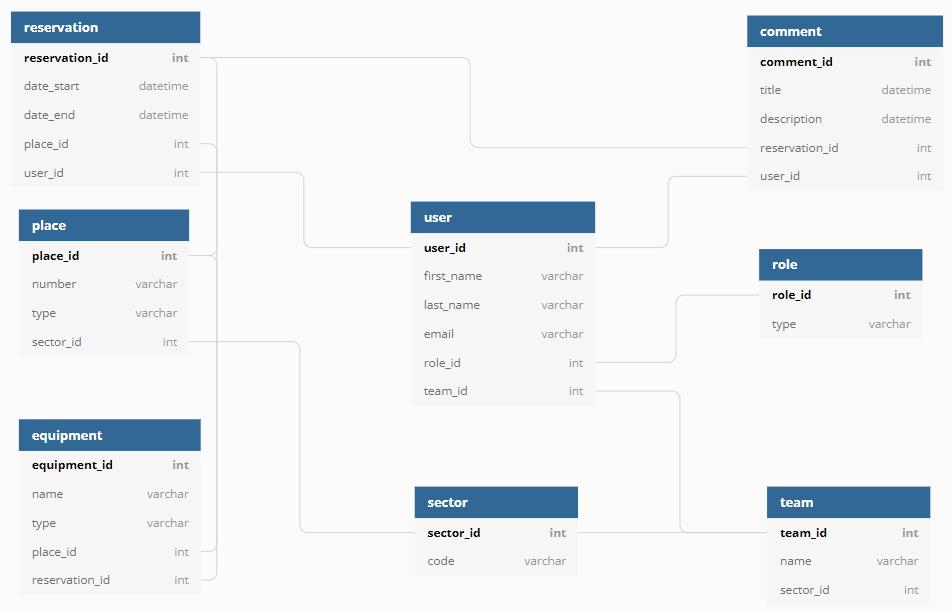
\includegraphics[scale=0.6]{db_diagram}
\begin{center}\textbf{Rys.7} Diagram struktury bazy danych \end{center}
Schemat relacyjnej bazy danych składa się z 8 tabel. Głowną tabelą jest tabela reservation, która zawiera w sobie tylko daty rezerwacji a następnie jest powiązana z danym miejscem, użytkownikiem, dodatkowym sprzętem oraz sekcją komentarzy. Każde miejsce znajduje się w pewnym sektorze (np. piętra). Użytkownik ma przypisaną rolę oraz zespół do którego należy.


\section{Słownik pojęć}
\begin{itemize}
  \item Rezerwacja - wpis o zajętym stanie danego miejsca wraz z podstawowymi informacjami o niej (termin, miejsce) oraz dodatkowych (dodatkowe wyposażenie)
  \item Administrator - rola w systemie, która ma wgląd do admin panelu pozwalającego na wgląd do statystyk, zarządzanie systemem i sprawdzenie jego stanu oraz generację raportu
  \item Raport - dokument, który zawiera stan rezerwacji z danego tygodnia
  \item Statystyka - zbiór metryk z rezerwacji i innych dodatkowych informacji prezentowanych na wykresach
\end{itemize}


\end{document}
